% =====================================================================
% EE 311 Midterm Report (IEEE journal format)
% Compile with pdflatex, or upload this file and the figures/ folder to Overleaf.
% =====================================================================
\documentclass[journal]{IEEEtran}

\usepackage[T1]{fontenc}
\usepackage[utf8]{inputenc}
\usepackage{cite}
\usepackage{booktabs}
\usepackage{tabularx}
\usepackage{graphicx}
\usepackage{url}

\newcommand{\authorname}{Oğuz Kağan Göçmez}

\begin{document}

\title{Machine Learning Prediction of Heating and Cooling Loads of Residential Buildings\\[0.3em]
{\LARGE Midterm Report}}

\author{\authorname%
\thanks{The author is with Özyeğin University, İstanbul, Türkiye.
This report is part of the EE~311 Introduction to Artificial Intelligence,
Machine Learning and Data Science course project, Fall 2026.}}

\maketitle

% ---------------------------------------------------------------------
\begin{abstract}
This project predicts the heating load (HL) and cooling load (CL) of residential buildings from eight
design parameters, using the UCI Energy Efficiency dataset of 768 buildings simulated in Ecotect.
Following the reference study of Tsanas and Xifara, the data were analyzed statistically, six regression
models were compared using 10-fold cross-validation (CV) repeated 10 times, and the three most promising
models were tuned. Tuned gradient boosting gave the lowest errors, with a mean absolute error (MAE) of
0.21 for HL and 0.41 for CL in a nested CV check, compared with 0.51 and 1.42 for the random forest of the
reference study.

As an additional contribution, the models were also tested on building shapes not seen during training,
using leave-one-shape-out CV. In this setting, the best MAE increased to 3.46 for HL and 3.75 for CL, and
the simplest models (linear regression and $k$-nearest neighbors) performed best. Tuning the models with
the same grouped CV reduced these errors to 3.11 and 3.26. The results show that random-split CV mainly
measures performance on building shapes that are already in the training data.
\end{abstract}

\begin{IEEEkeywords}
Building energy performance, heating load, cooling load, machine learning, regression, cross-validation.
\end{IEEEkeywords}

% ---------------------------------------------------------------------
\section{Introduction}
\IEEEPARstart{H}{VAC} systems account for most of the energy used in buildings, so estimating heating
and cooling loads in the early design phase supports the design of energy-efficient
buildings~\cite{tsanas2012}. Simulation tools provide reliable estimates but are time-consuming, which
has motivated the use of ML models such as decision trees~\cite{yu2010}, support vector
machines~\cite{dong2005} and polynomial regression~\cite{catalina2008}. Tsanas and
Xifara~\cite{tsanas2012} introduced the dataset used in this project~\cite{uci2012} and reported MAE
values of 0.51 for HL and 1.42 for CL with a random forest (RF).

This report describes the work completed since the project plan, following the Machine Learning Project
Checklist of the course textbook~\cite{geron2022}, and presents the remaining work and the revised
schedule. Table~\ref{tab:status} summarizes the status of each subtask.

% ---------------------------------------------------------------------
\section{Work Accomplished So Far}

\begin{table}[!h]
\caption{Status of the Subtasks}
\label{tab:status}
\centering
\begin{tabularx}{\columnwidth}{@{}Xl@{}}
\toprule
Subtask & Status \\
\midrule
Literature search               & Done \\
Frame the problem               & Done \\
Get the data                    & Done \\
Explore the data                & Done \\
Prepare the data                & Basic version done \\
Shortlist promising models      & Done \\
Grouped CV by building shape    & Done \\
Fine-tune the system            & Done (final run pending) \\
Feature importance              & Partly done \\
Present the results             & Planned \\
\bottomrule
\end{tabularx}
\end{table}

\subsection{Literature Search}
In addition to the reference study~\cite{tsanas2012}, four studies on the same dataset were reviewed.
Castelli \emph{et al.}~\cite{castelli2015} used genetic programming with the same evaluation protocol as
the reference study and reported MAE values of 0.51 for HL and 1.18 for CL. \v{Z}egklitz and
Po\v{s}\'{\i}k~\cite{zegklitz2017} compared symbolic regression methods with a tuned RF and support vector
regression (SVR) and reported a median test root mean squared error (RMSE) of 0.51 for HL (RF) and 1.28
for CL (SVR); their results suggested that a tuned SVR is worth considering for CL. Yazici
\emph{et al.}~\cite{yazici2018} used the dataset to test ML models on a low-power Internet of Things
device and found the RF to be the most accurate model. Sajjad \emph{et al.}~\cite{sajjad2020} proposed a
recurrent neural network that predicts both loads together. However, several of their reported results
are inconsistent; for example, some rows report an RMSE smaller than the MAE, which is not possible.
Their numbers were therefore not used for comparison. The main lesson from this step was that results
from the literature should be checked before they are compared, since the papers use different
protocols and error measures.

\subsection{Data Collection and Exploration}
The dataset~\cite{uci2012} contains 768 buildings and 10 columns: eight inputs (relative compactness,
surface area, wall area, roof area, overall height, orientation, glazing area, and glazing area
distribution) and two outputs (HL and CL). It was loaded from a CSV export of the original Excel file and
checked against it; there are no missing values and no duplicate rows. The buildings are generated from
12 shapes, each combined with 4 orientations and 16 glazing options, so each shape appears 64 times.

The association of each input with each output was measured with mutual information and the Spearman rank
correlation, as in~\cite{tsanas2012}. The Spearman correlation was used instead of the Pearson correlation
because the variables are not normally distributed. Fig.~\ref{fig:heatmap} shows the Spearman correlation
between all variables. Overall height ($\rho=0.86$) and roof area ($\rho=-0.80$) are the inputs most
strongly related to both loads, and HL and CL are themselves strongly correlated ($\rho=0.97$). Relative
compactness and surface area are perfectly rank-correlated ($\rho=-1$), so they carry the same
information. Orientation is not correlated with either output ($|\rho| \leq 0.02$, $p>0.6$).

A closer look showed that orientation still matters in some cases. For each group of four buildings that
differ only in orientation, the change in load was computed. For HL and for most shapes, the median change
is small (at most about 1.6). For the CL of four two-storey shapes, however, the median change is between
about 4 and 9, and the effect does not go in one direction, which explains why the correlation is close
to zero. The lesson is that a correlation of zero does not prove that an input has no effect.

\begin{figure}[!tb]
\centering
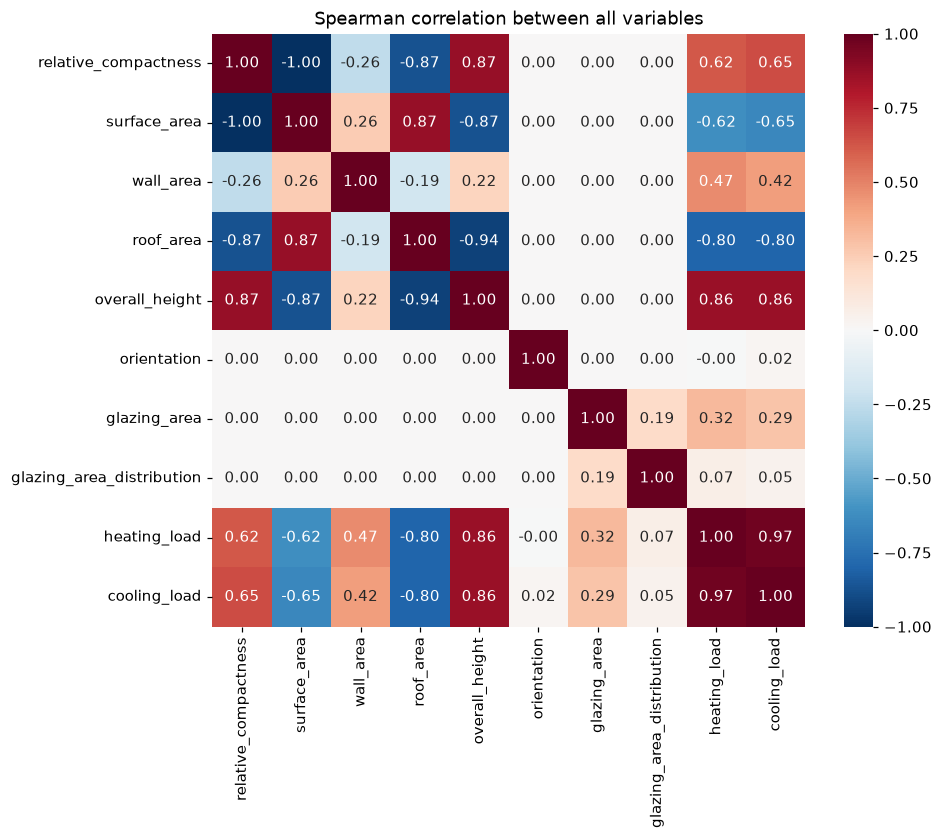
\includegraphics[width=\columnwidth]{figures/correlation_heatmap.png}
\caption{Spearman rank correlation between all inputs and outputs.}
\label{fig:heatmap}
\end{figure}

\subsection{Data Preparation}
The data required no cleaning, since there are no missing values, text columns or duplicate rows. The
inputs of the models that are sensitive to scale (robust linear regression, $k$-nearest neighbors and
SVR) were standardized inside a pipeline. In this way, the scaler is fitted on the training folds only,
and no information from the test fold is used during training.

\subsection{Model Shortlisting}
Six models implemented in scikit-learn~\cite{pedregosa2011} were compared with default settings: linear
regression, robust linear regression with the Huber loss (a robust alternative comparable to the IRLS model
of~\cite{tsanas2012}), $k$-nearest neighbors, SVR, RF~\cite{breiman2001}, and gradient
boosting~\cite{friedman2001}. Each model was evaluated with 10-fold CV repeated 10 times, using the three
error measures of~\cite{tsanas2012}: MAE, mean squared error (MSE), and mean relative error (MRE).

Table~\ref{tab:shortlist} and Fig.~\ref{fig:models} show the MAE of each model. The tree-based models
performed best, with the RF reaching an MAE of 0.31 for HL and 0.98 for CL, which is already lower than
the RF of the reference study. The linear models gave errors close to those of the IRLS model
in~\cite{tsanas2012}. As in the reference study, CL was harder to predict than HL for all models.

\begin{table}[!tb]
\caption{Untuned Models: MAE (Mean $\pm$ Std), 10-Fold CV Repeated 10 Times}
\label{tab:shortlist}
\centering
\begin{tabular}{@{}lcc@{}}
\toprule
Model & Heating load & Cooling load \\
\midrule
Linear regression           & $2.09 \pm 0.24$ & $2.27 \pm 0.27$ \\
Robust linear (Huber)       & $2.03 \pm 0.25$ & $2.20 \pm 0.30$ \\
$k$-nearest neighbors       & $1.42 \pm 0.20$ & $1.66 \pm 0.24$ \\
Support vector regression   & $0.55 \pm 0.08$ & $1.13 \pm 0.19$ \\
Gradient boosting           & $0.34 \pm 0.04$ & $1.02 \pm 0.13$ \\
Random forest               & $\mathbf{0.31 \pm 0.04}$ & $\mathbf{0.98 \pm 0.14}$ \\
\midrule
IRLS in~\cite{tsanas2012}   & $2.14 \pm 0.24$ & $2.21 \pm 0.28$ \\
RF in~\cite{tsanas2012}     & $0.51 \pm 0.11$ & $1.42 \pm 0.25$ \\
\bottomrule
\end{tabular}
\end{table}

\begin{figure*}[!t]
\centering
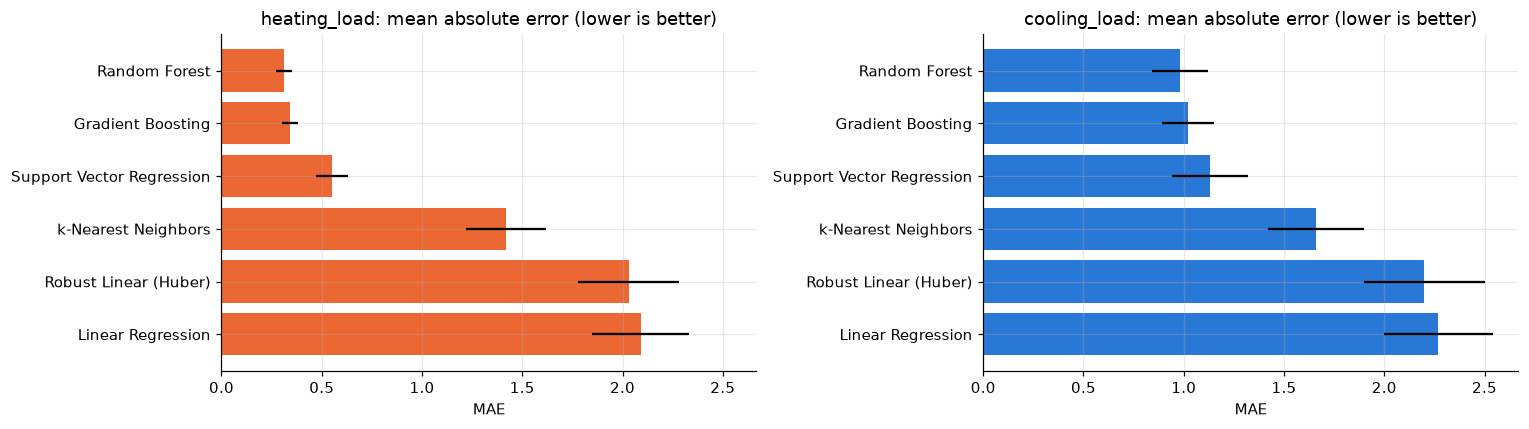
\includegraphics[width=\textwidth]{figures/model_comparison.png}
\caption{MAE of the untuned models (error bars: standard deviation over the CV folds).}
\label{fig:models}
\end{figure*}

\subsection{Fine-Tuning}
The three best models (RF, gradient boosting and SVR) were tuned separately for each load with a
randomized search that tried 40 hyperparameter settings per model, each scored by its MAE in 5-fold CV.
The tuned models were then evaluated with the same repeated 10-fold CV as before. Because the search and
the evaluation used the same data, the tuned errors may be slightly optimistic. To check this, a nested CV
was also performed, in which the search was repeated inside each of 10 outer training folds, so that the
search never saw the test fold.

Table~\ref{tab:tuned} shows the results. Tuning improved gradient boosting considerably, from 0.34 to 0.20
for HL and from 1.02 to 0.36 for CL, and it also improved SVR, whereas the RF did not benefit from tuning.
The nested errors agree with the tuned errors within 0.01, except for gradient boosting on CL (0.41 versus
0.36). The nested values are therefore reported as the fairer estimate: tuned gradient boosting reaches an
MAE of 0.21 for HL and 0.41 for CL, less than half of the errors of the RF in~\cite{tsanas2012}.

\begin{table}[!tb]
\caption{Tuned Models: MAE, Untuned $\rightarrow$ Tuned, and Nested-CV Check}
\label{tab:tuned}
\centering
\begin{tabular}{@{}lcccc@{}}
\toprule
& \multicolumn{2}{c}{Heating load} & \multicolumn{2}{c}{Cooling load} \\
Model & Tuned & Nested & Tuned & Nested \\
\midrule
Gradient boosting  & $0.34 \rightarrow \mathbf{0.20}$ & $\mathbf{0.21}$ & $1.02 \rightarrow \mathbf{0.36}$ & $\mathbf{0.41}$ \\
SVR                & $0.55 \rightarrow 0.34$ & $0.34$ & $1.13 \rightarrow 0.87$ & $0.87$ \\
Random forest      & $0.31 \rightarrow 0.32$ & $0.31$ & $0.98 \rightarrow 0.94$ & $0.95$ \\
\midrule
RF in~\cite{tsanas2012} & $0.51$ & & $1.42$ & \\
\bottomrule
\end{tabular}
\end{table}

\subsection{Generalization to Unseen Building Shapes}
Since buildings that differ only in orientation mostly have very similar loads, a random split places
near-copies of most test buildings in the training folds. A designer, however, would use the model for
a new building shape. To test this case, leave-one-shape-out CV was used~\cite{roberts2017}: each of the
12 folds holds out all 64 buildings of one shape, and the model is trained on the other 11 shapes.

Table~\ref{tab:unseen} compares the MAE on random splits with the MAE on unseen shapes. Every model
performed much worse on unseen shapes: the best MAE increased to 3.46 for HL and 3.75 for CL, which is
10 to 17 times the best random-split errors. The ranking was also reversed: the linear models and
$k$-nearest neighbors, the weakest models under random CV, became the best, while the tree models
performed worse, and SVR tuned for random CV reached an MAE above 16. An analysis of the error on each shape
showed that some shapes are easy and others very hard. For example, the tree models failed on shape 0.74,
because its compactness and surface area lie at the border between the one-storey and two-storey shapes,
so trees that split on these inputs grouped it with the two-storey buildings.

When the hyperparameters were tuned with the same grouped CV, the best errors decreased to 3.11 for HL
(SVR) and 3.26 for CL ($k$-nearest neighbors). The grouped search selected much simpler settings for SVR,
which shows that the tuning procedure should match the intended use of the model.

\begin{table}[!tb]
\caption{MAE on Random Splits vs.\ Unseen Building Shapes (Leave-One-Shape-Out CV)}
\label{tab:unseen}
\centering
\begin{tabular}{@{}lcccc@{}}
\toprule
& \multicolumn{2}{c}{Heating load} & \multicolumn{2}{c}{Cooling load} \\
Model & Random & Unseen & Random & Unseen \\
\midrule
Linear regression          & 2.09 & 3.51 & 2.27 & 3.93 \\
Robust linear (Huber)      & 2.03 & 3.49 & 2.20 & \textbf{3.75} \\
$k$-nearest neighbors      & 1.42 & \textbf{3.46} & 1.66 & 3.93 \\
Random forest              & 0.31 & 4.26 & 0.98 & 4.95 \\
Gradient boosting (tuned)  & 0.20 & 5.26 & 0.36 & 4.79 \\
SVR (tuned)                & 0.34 & 17.85 & 0.87 & 16.90 \\
\bottomrule
\end{tabular}
\end{table}

\subsection{Input Importance}
The built-in feature importance of an RF trained on all the data was examined. The shape-related inputs
(relative compactness or surface area, roof area and overall height) received most of the importance,
and orientation received almost none, in agreement with the correlation analysis. Unlike the reference
study, glazing area was not the most important input. Since~\cite{tsanas2012} used a different importance
measure, this difference will be examined further with permutation importance.

% ---------------------------------------------------------------------
\section{Remaining Work}
The following work remains. As this is a single-author project, the author is responsible for all of it.
\begin{itemize}
\item \emph{Final results:} repeat the evaluation with 100 CV repetitions, as in~\cite{tsanas2012}, and
report all three error measures.
\item \emph{Input importance:} compute the permutation importance of the tuned models and add a random
probe feature, as in~\cite{tsanas2012}, to examine the difference in the importance of glazing area.
\item \emph{Redundant inputs:} remove relative compactness or surface area, and test whether this fixes the
failure of the tree models on unseen shapes such as 0.74.
\item \emph{Encoding:} encode orientation and glazing area distribution as categories (one-hot encoding)
and test whether the linear models improve.
\item \emph{Multi-output model:} test a single model that predicts both loads, since they are strongly
correlated.
\item \emph{Reporting:} prepare the final tables and figures, the final report and the recorded
presentation.
\end{itemize}

% ---------------------------------------------------------------------
\section{Revised Project Plan}
Table~\ref{tab:schedule} shows the revised schedule. Compared with the project plan, model shortlisting,
fine-tuning and the grouped-CV analysis were completed earlier than planned. The midterm report, however,
was delayed from Week~4 to Week~6, and the remaining analyses were moved to Week~6 so that the final report
and the presentation can be completed in Week~7, the last week of the semester.

\begin{table}[!h]
\caption{Revised Project Schedule}
\label{tab:schedule}
\centering
\begin{tabularx}{\columnwidth}{@{}Xc@{}}
\toprule
Subtask & Week \\
\midrule
Literature search               & 1--2 \\
Frame the problem               & 1    \\
Get the data                    & 1    \\
Explore the data                & 2    \\
\textbf{Project plan report}    & 2    \\
Prepare the data                & 3    \\
Shortlist promising models      & 3    \\
Grouped CV by building shape    & 4    \\
Fine-tune the system            & 5    \\
\textbf{Midterm report}         & 6    \\
Final run and remaining analyses & 6   \\
Present the results             & 6--7 \\
\textbf{Final report}           & 7    \\
\textbf{Recorded presentation}  & 7    \\
\bottomrule
\end{tabularx}

\vspace{2pt}
\footnotesize Week~1 begins on October~19, 2026, and Week~7 (beginning on November~30, 2026)
is the last week of the semester.
\end{table}

% ---------------------------------------------------------------------
\section*{Acknowledgment}
% Check this paragraph after rephrasing the report, and keep it accurate.
An AI tool (Claude, Anthropic) was used in this project, with the permission of the course instructor.
It suggested methods, namely the use of the Spearman correlation and a list of candidate regression
models, which the author verified against the literature before deciding which ones to use. It also
produced a draft of the text of this report from the author's results, which the author then reviewed,
checked against the results and rewrote. The analysis code was written by the author. All AI suggestions
were carefully reviewed by the author, and their correctness was validated.

% ---------------------------------------------------------------------
\begin{thebibliography}{13}

\bibitem{tsanas2012}
A.~Tsanas and A.~Xifara, ``Accurate quantitative estimation of energy performance of residential
buildings using statistical machine learning tools,'' \emph{Energy Build.}, vol.~49, pp.~560--567,
2012, doi: 10.1016/j.enbuild.2012.03.003.

\bibitem{yu2010}
Z.~Yu, F.~Haghighat, B.~C.~M. Fung, and H.~Yoshino, ``A decision tree method for building energy
demand modeling,'' \emph{Energy Build.}, vol.~42, no.~10, pp.~1637--1646, 2010,
doi: 10.1016/j.enbuild.2010.04.006.

\bibitem{dong2005}
B.~Dong, C.~Cao, and S.~E. Lee, ``Applying support vector machines to predict building energy
consumption in tropical region,'' \emph{Energy Build.}, vol.~37, no.~5, pp.~545--553, 2005,
doi: 10.1016/j.enbuild.2004.09.009.

\bibitem{catalina2008}
T.~Catalina, J.~Virgone, and E.~Blanco, ``Development and validation of regression models to predict
monthly heating demand for residential buildings,'' \emph{Energy Build.}, vol.~40, no.~10,
pp.~1825--1832, 2008, doi: 10.1016/j.enbuild.2008.04.001.

\bibitem{uci2012}
A.~Tsanas and A.~Xifara, ``Energy Efficiency,'' UCI Machine Learning Repository, 2012.
[Online]. Available: \url{https://doi.org/10.24432/C51307}

\bibitem{castelli2015}
M.~Castelli, L.~Trujillo, L.~Vanneschi, and A.~Popovi\v{c}, ``Prediction of energy performance of
residential buildings: A genetic programming approach,'' \emph{Energy Build.}, vol.~102, pp.~67--74,
2015, doi: 10.1016/j.enbuild.2015.05.013.

\bibitem{zegklitz2017}
J.~\v{Z}egklitz and P.~Po\v{s}\'{\i}k, ``Symbolic regression algorithms with built-in linear
regression,'' 2017, arXiv:1701.03641. [Online]. Available: \url{https://arxiv.org/abs/1701.03641}

\bibitem{yazici2018}
M.~T. Yazici, S.~Basurra, and M.~M. Gaber, ``Edge machine learning: Enabling smart Internet of Things
applications,'' \emph{Big Data Cogn. Comput.}, vol.~2, no.~3, Art. no.~26, 2018,
doi: 10.3390/bdcc2030026.

\bibitem{sajjad2020}
M.~Sajjad \emph{et al.}, ``Towards efficient building designing: Heating and cooling load prediction
via multi-output model,'' \emph{Sensors}, vol.~20, no.~22, Art. no.~6419, 2020,
doi: 10.3390/s20226419.

\bibitem{geron2022}
A.~G\'{e}ron, \emph{Hands-On Machine Learning with Scikit-Learn, Keras, and TensorFlow}, 3rd~ed.
Sebastopol, CA, USA: O'Reilly Media, 2022.

\bibitem{pedregosa2011}
F.~Pedregosa \emph{et al.}, ``Scikit-learn: Machine learning in Python,'' \emph{J. Mach. Learn. Res.},
vol.~12, pp.~2825--2830, 2011. [Online]. Available: \url{https://jmlr.org/papers/v12/pedregosa11a.html}

\bibitem{breiman2001}
L.~Breiman, ``Random forests,'' \emph{Mach. Learn.}, vol.~45, no.~1, pp.~5--32, 2001,
doi: 10.1023/A:1010933404324.

\bibitem{friedman2001}
J.~H. Friedman, ``Greedy function approximation: A gradient boosting machine,''
\emph{Ann. Statist.}, vol.~29, no.~5, pp.~1189--1232, 2001, doi: 10.1214/aos/1013203451.

\bibitem{roberts2017}
D.~R. Roberts \emph{et al.}, ``Cross-validation strategies for data with temporal, spatial,
hierarchical, or phylogenetic structure,'' \emph{Ecography}, vol.~40, no.~8, pp.~913--929, 2017,
doi: 10.1111/ecog.02881.

\end{thebibliography}

\end{document}
